\section{Coupled sea-level alternatives and tail coverage}
\subsection{Sampling rare emissions without changing their probability}
The balanced 256-member calculation contains no warming above 3.5 K. To examine
rare emissions without altering their probability, we partition the same
10,000 prior trajectories into five strata. These contain 235 budget-compliant
draws, 9,265 remaining draws through the overall 95th percentile, 400 between
the 95th and 99th percentiles, 90 between the 99th and 99.9th percentiles, and
10 above the 99.9th percentile. We sample 96, 64, 48, 32 and 10 trajectories,
respectively, without replacement. The prior and both budget alternatives
retain their empirical stratum masses. Complete climate-parameter rows are
paired independently with these emissions draws.

The initial eight-member tail pilot fails the declared 0.001 ppm CO$_2$
refinement criterion: doubling eight to sixteen substeps changes CO$_2$ by
0.001908 ppm. We retain that failed result and double the working resolution.
The revised sixteen-versus-thirty-two-substep pilot changes temperature by at
most $9.08\times10^{-6}$ K and CO$_2$ by $4.77\times10^{-4}$ ppm. Carbon mass
closes within $8.19\times10^{-12}$ Gt C. The subsequent 250-member experiment
uses sixteen substeps and takes 512 wall seconds on one thread.

The four warming categories contain 107, 65, 73 and 5 members. Under the 50\%
budget alternative, their probabilities are 58.81\%, 33.35\%, 7.78\% and
0.0534\%. The last category's conditional effective sample size is only 4.23;
its endpoints cannot establish converged 5th or 95th percentiles. Tail sampling
therefore resolves the earlier absence of high warming as a finite-sample
limitation, but does not recover the published warming probabilities.

\subsection{Component assembly and Antarctic shore feedback}
BRICK's written description supplies Antarctic-shore factors of $-1$ for the
Antarctic contribution and $+1$ for other components, together with previous-year
forcing in its annual coupling\cite{brick}. These local factors permit a shore
feedback calculation without inventing global fingerprint maps. If $A$ is the
Antarctic global contribution and $O$ is the sum of other contributions, the
shore level is
\begin{equation}
 S_{\rm shore}(t)=S_{\rm shore}(t_0)+O(t)-A(t),
 \qquad O(t_0)=A(t_0)=0.
\end{equation}
We evolve Antarctic volume and invert its verified geometric relation at each
stage. A separate radius-coordinate integration includes the resulting
sea-level derivative and agrees with the volume calculation. Continuous
stagewise feedback is an explicitly derived alternative; freezing the forcing
at the previous annual knot tests the documented lag convention.

The future budget combines conditional glacier and Greenland parameter rows,
the Antarctic point fits, thermosteric change and land-water storage. The
Antarctic splice begins at the final paleo-forcing knot, 2009.5, and subsequent
shore changes follow the equation above. Glacier and Greenland histories use
observed temperature through 2021. Future forcing retains the observed boundary
temperature before joining the modeled series. Storage has a documented mean
rate of 0.30 mm yr$^{-1}$ and standard deviation 0.18 mm yr$^{-1}$; Gaussian
independent annual rates and a common uncertain rate are separate assumptions.
Thermosteric alternatives apply the independently fitted 0--2000 m coefficient
either to that depth alone or to the full modeled ocean heat change. Neither
alternative recovers a full-depth target posterior.

Five closure choices and two non-CO$_2$ forcing rules give 2,500 member cases.
The initial pilot checks halved Antarctic timesteps and component sums before
the 250-member extension. The base experiment produces 0.111--1.448 m of global
change by 2100 relative to 2010. This is an \emph{uncorrected alternative budget}:
the observational peripheral-glacier overlap, conditional parameter fits and
omitted cross-component dependence remain explicit limitations.

\begin{figure}[htbp]
\centering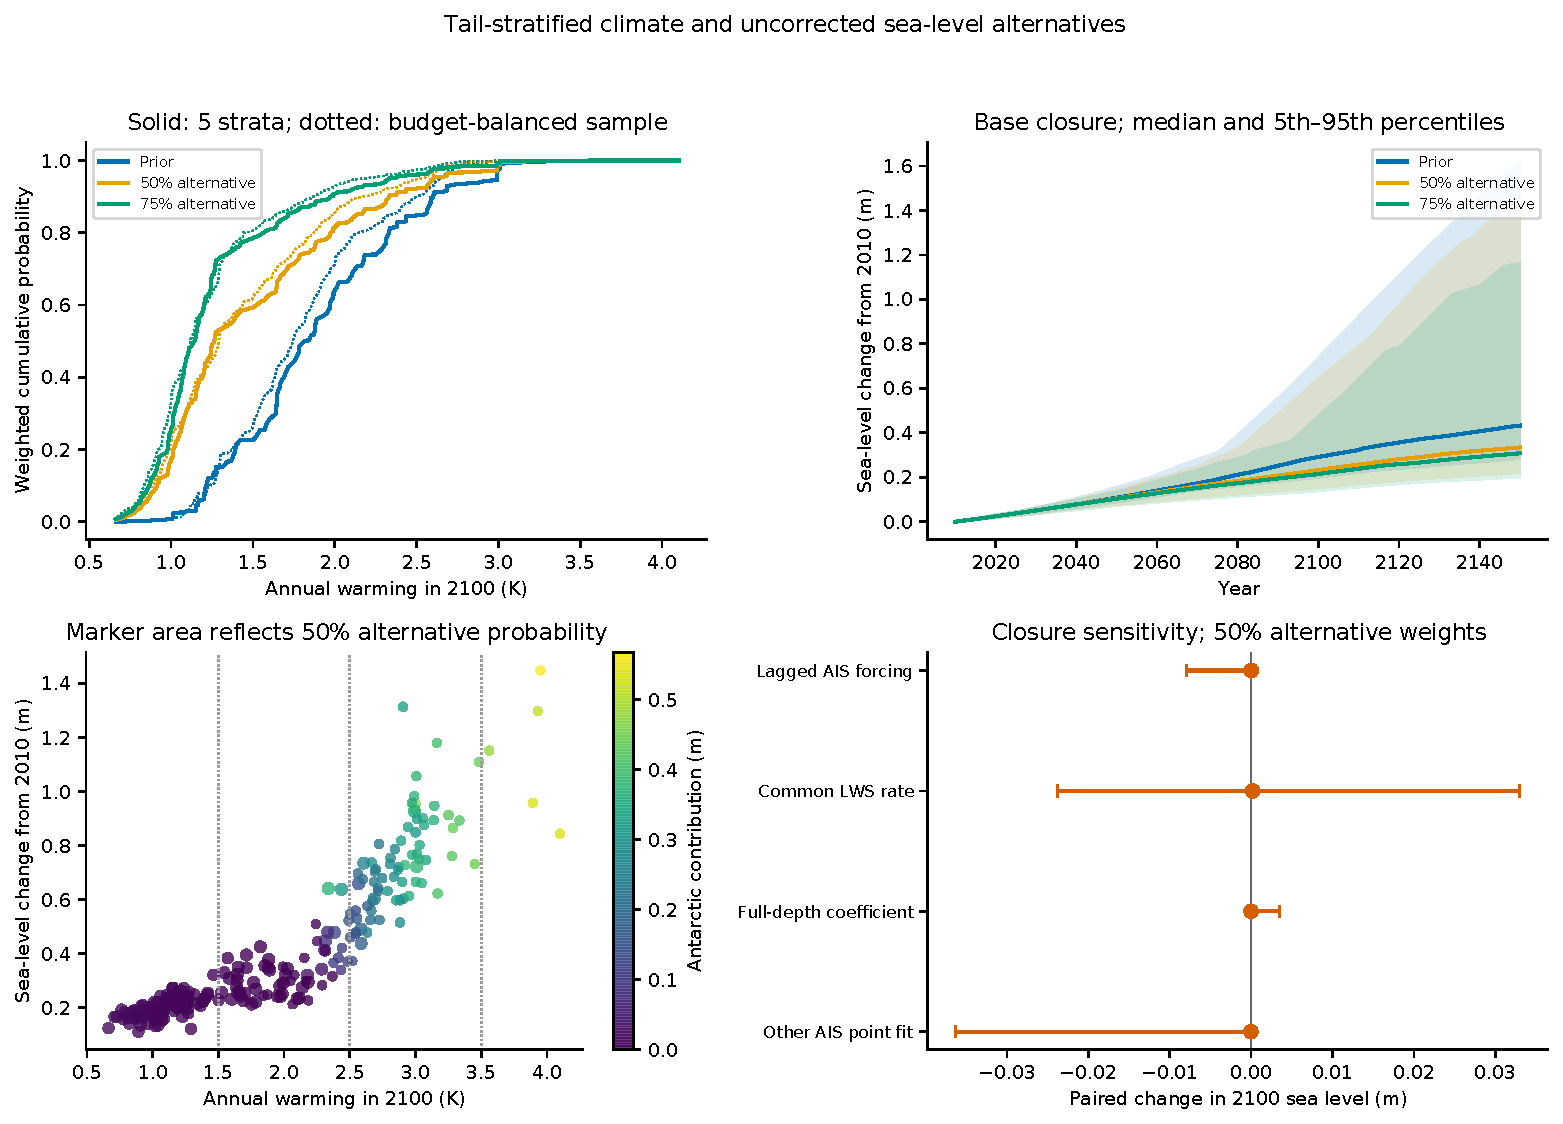
\includegraphics[width=\linewidth]{figures/coupled_sea_level_alternatives.pdf}
\caption{Tail sampling and coupled sea-level alternatives. Upper left:
weighted warming distributions for the five-stratum experiment (solid) and
the earlier balanced experiment (dotted). Upper right: base sea-level medians
and 5th--95th percentiles. Lower left: member-level warming and sea level;
color denotes the Antarctic contribution and marker size reflects alternative
probability weight. Lower right: paired 2100 closure differences, using 50\%
budget weights. These are independent sensitivity experiments, not recovered
published distributions.}\label{fig:seacoupled}
\end{figure}

The two Antarctic fits satisfy almost identical paleo constraints but differ
by as much as 0.363 m in their future contribution. The fitted fast-loss
threshold and rate therefore remain consequential beyond the calibration
windows. Changing the storage covariance shifts individual 2100 totals by up
to 0.050 m; the full-depth thermal alternative changes them by up to 0.025 m;
lagging Antarctic forcing changes them by up to 0.011 m. These are sensitivities
to named choices, not bounds on total scientific uncertainty.

\subsection{Reference-period recovery and AR6 context}
We recover the model's own 1995--2014 reference by combining its historical
component calculations with the saved 2010--2014 forward segment. Each member's
twenty annual values are averaged before subtracting that mean. The datum shift
is 0.0071--0.0183 m and is not fitted to an external projection. On this datum,
the 50\% budget alternative has a 2100 median of 0.244 m and a 17th--83rd range
of 0.194--0.363 m. The corresponding prior values are 0.304 m and
0.242--0.491 m.

AR6 Table 9.9 reports a 2100 median and likely range of 0.56 (0.44--0.76) m for
SSP2-4.5\cite{ar6sea}. The independent alternatives remain lower after matching
the reference period. However, their emissions distributions are different;
this is a contextual comparison, not a matched-scenario validation. Conditional
ice fits, the low inferred climate sensitivity and missing joint uncertainty
can all affect this comparison. We do not adjust any component to match AR6.

\begin{figure}[htbp]
\centering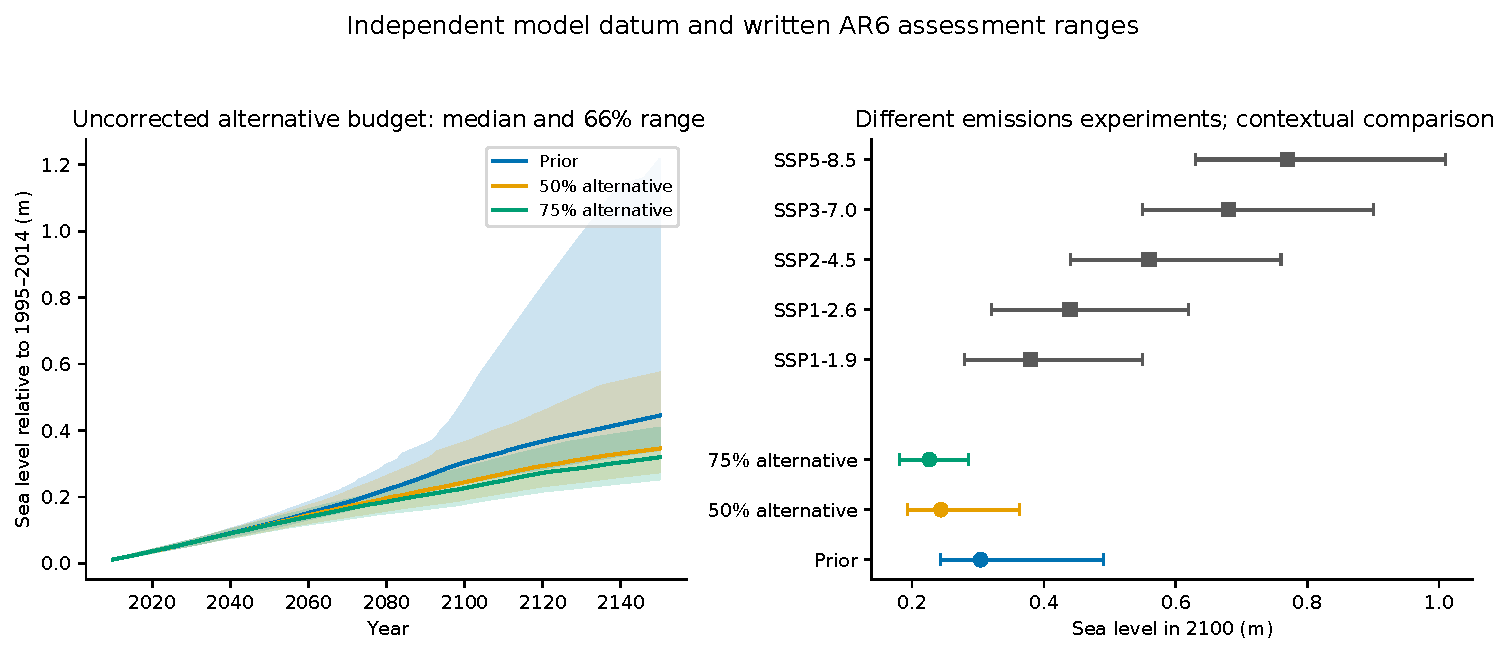
\includegraphics[width=\linewidth]{figures/sea_level_ar6_context.pdf}
\caption{Datum-consistent sea-level context for supplementary Figure 4.
Left: independent alternative medians and 17th--83rd percentiles relative to
each member's 1995--2014 mean. Right: 2100 alternative ranges and printed AR6
Table 9.9 SSP ranges on the same datum. The SSP scenarios and probabilistic
emissions alternatives are distinct experiments. The written AR6 summary values
are comparison evidence only and are not inputs to the model.}
\label{fig:seaar6}
\end{figure}
